\iffalse 

TODO : 
参考文献修正、フッターに書く?
リストのマークを変える、サイズ大きく
本文文字太くする?
画像があるといい

\fi

\RequirePackage{plautopatch} 
\documentclass[17pt]{beamer} 
\usepackage{amsmath}
\usepackage{amssymb}
\usepackage{graphicx}
\usepackage{luatexja}
\usepackage{luatexja-fontspec} 
\usepackage{fontspec}
\usepackage{color} 
\usepackage{tcolorbox}
\usepackage{ascmac}
\usepackage{bm} 
\usepackage{appendixnumberbeamer}
\usepackage{comment}
\usepackage[absolute,overlay]{textpos}

\usepackage{enumitem}
\setlist[itemize,1]{label=\textbullet, itemsep=17pt}  % 記号をもうちょっと大きくしたい
\setlist[itemize,2]{label=\textendash, itemsep=3pt} 
\setlist[itemize,3]{label=\textendash, itemsep=3pt} 

\usetheme{metropolis}  % Metropolisテーマを使用
\setmainjfont{Yu Gothic Bold}  
\setsansjfont{Yu Gothic Bold}  

%Beamerフォント設定 
\usefonttheme{professionalfonts} % Be professional!
\usepackage[T1]{fontenc}
\usepackage{mlmodern}  % 太いComputer Modern
% MLmodernのバグを修正: cf. https://tex.stackexchange.com/questions/646333/size-of-integral-symbol-in-section-header-with-mlmodern
\DeclareFontFamily{OMX}{mlmex}{}
\DeclareFontShape{OMX}{mlmex}{m}{n}{%
   <->mlmex10%
   }{} 
\renewcommand{\familydefault}{\sfdefault}  % 英文をサンセリフ体に
\renewcommand{\kanjifamilydefault}{\gtdefault}  % 日本語をゴシック体に
\usefonttheme{structurebold} % タイトル部を太字
\setbeamerfont{alerted text}{series=\bfseries} % Alertを太字
\setbeamerfont{section in toc}{series=\mdseries} % 目次は太字にしない
\setbeamerfont{frametitle}{size=\large} % フレームタイトル文字サイズ
\setbeamerfont{title}{size=\Large} % タイトル文字サイズ
\setbeamerfont{date}{size=\normalsize}  % 日付文字サイズ
\setbeamerfont{author}{size=\normalsize}  % 日付文字サイズ
\setbeamerfont{normal text}{series=\mdseries} % 本文を太字に 

%ページ番号の設定
\setbeamertemplate{footline}{
    \hfill {\textcolor{gray!90}{\insertframenumber/\inserttotalframenumber}\hspace{0.1cm}}
    \vspace{0.1cm} 
}

\setlength{\leftmargini}{0.1cm} % itemizeのマージンを詰める
\makeatletter\setlength{\metropolis@frametitle@padding}{1.4ex}%タイトルの余白

%短縮形
\newcommand{\Pbb}{\mathbb{P}}
\newcommand{\Gcal}{\mathcal{G}}
\newcommand{\Fcal}{\mathcal{F}}

%タイトル
\title{¬ACの相対的無矛盾性証明のIsabelle/ZFによる形式化}
\author{東北大学 大学院情報科学研究科\\ 住井・松田研究室 M2\\ 舟根大喜}
\date{November 22, 2024}

\begin{document}
\maketitle

\begin{frame}{概要}
    \vspace{-5pt}
    \begin{itembox}[l]{やったこと}
        \begin{center}
        \vspace{-3pt}
        $\neg$ACのZF上の相対的無矛盾性証明を\\
        Isabelle/ZFで形式化
        \vspace{-3pt}
        \end{center}
    \end{itembox}
    \vspace{-5pt}
    {\small
    \textcolor{red}{動機}
    \begin{itemize}[itemsep=1pt]
    \vspace{-5pt}
        \item 定理証明支援系を用いて\\
        数学の形式化をする試みが行われている
        \item 公理的集合論の重要な技法である強制法(後述)を用いた議論の形式化は限られている
        \item ACの相対的無矛盾性証明は形式化されている\\
        ので合わせてACの独立性が形式化されたことになる
    \end{itemize}}
\end{frame}

\begin{frame}{用語}\,
    \vspace{-20pt}
    {\small 
        \begin{itemize}[itemsep=8pt]
            \item \textcolor{red}{公理的集合論} : \\
            集合がみたすべき性質を公理として定めた集合論
            \item \textcolor{red}{ZF} : 
            Zermelo-Fraenkel公理系。一階述語論理上で\\
            形式化されたよく採用される公理系
            \item \textcolor{red}{AC} \ldots 選択公理 (Axiom of Choice)\\
            任意の非空集合の族からそれぞれ1つの元を選ぶ関数が存在するという公理
            \begin{itemize}
                \item 整列可能定理、Zornの補題など\\同値な重要な命題がある
            \end{itemize}

        \end{itemize}
    }
\end{frame}

\begin{frame}{用語}\,
    \vspace{-20pt}
    {\small 
        \begin{itemize}[itemsep=8pt]
            \item 命題$\varphi$が公理系$T$上で\textcolor{red}{相対的無矛盾} :\\
            $T$が無矛盾ならば公理系$T+\varphi$も無矛盾なこと
            \item $\varphi$が$T$から\textcolor{red}{独立} : \\
            $T$から$\varphi$も$\neg\varphi$も証明できないこと   
        \end{itemize}

        \begin{itemize}
            \item [\textcolor{red}{$\blacktriangleright$}]
            $\varphi$と$\neg\varphi$のT上の相対的無矛盾性を示すことで\\
            $\varphi$が$T$から独立であることが証明できる\\
            ($T$が無矛盾と仮定すれば)
        \end{itemize}
    }
\end{frame}

\begin{frame}{用語}\,
    \vspace{-45pt}
    
    {\small 
    \begin{itemize}[itemsep=8pt]
        \item \textcolor{red}{強制法} : \\
        集合論のモデルを拡張し新しいモデルを作る技法
        \begin{itemize}
            \item $M$を強制法で拡張したモデルを\\$M$の\textcolor{red}{generic extension}と呼び$M[G]$と書く
            \item $M[G]$はposet $\Pbb$とgeneric filter $G$に依存しており、
            $\Pbb$をうまく選ぶことで、ある程度
            $M[G]$で成り立つことを制御できる
            \item $\Pbb$を決めたうえで、強制関係\textcolor{red}{$\Vdash$}によって、$M[G]$で成り立つことを確認できる
        \end{itemize}
    \end{itemize}
    \vspace{-15pt}
    ※モデルが存在すれば無矛盾であるため、
    強制法でモデルを構成することで無矛盾性を証明できる
}
\end{frame}
\section{Isabelle/ZFについて}

\begin{frame}{定理証明支援系}
    \begin{columns}
        \begin{column}{0.65\textwidth}
            {\small
            \begin{itemize}[itemsep=7pt]
                \item 数学的証明の形式化や、\\ソフトウェアの正しさの証明\\などに用いられるシステム
                \item プログラムを書くように\\定義・証明を記述する
                \item Isabelle,Lean,Coq, \ldots
            \end{itemize}
            }
        \end{column}
        \begin{column}{0.35\textwidth}
            \begin{figure}
                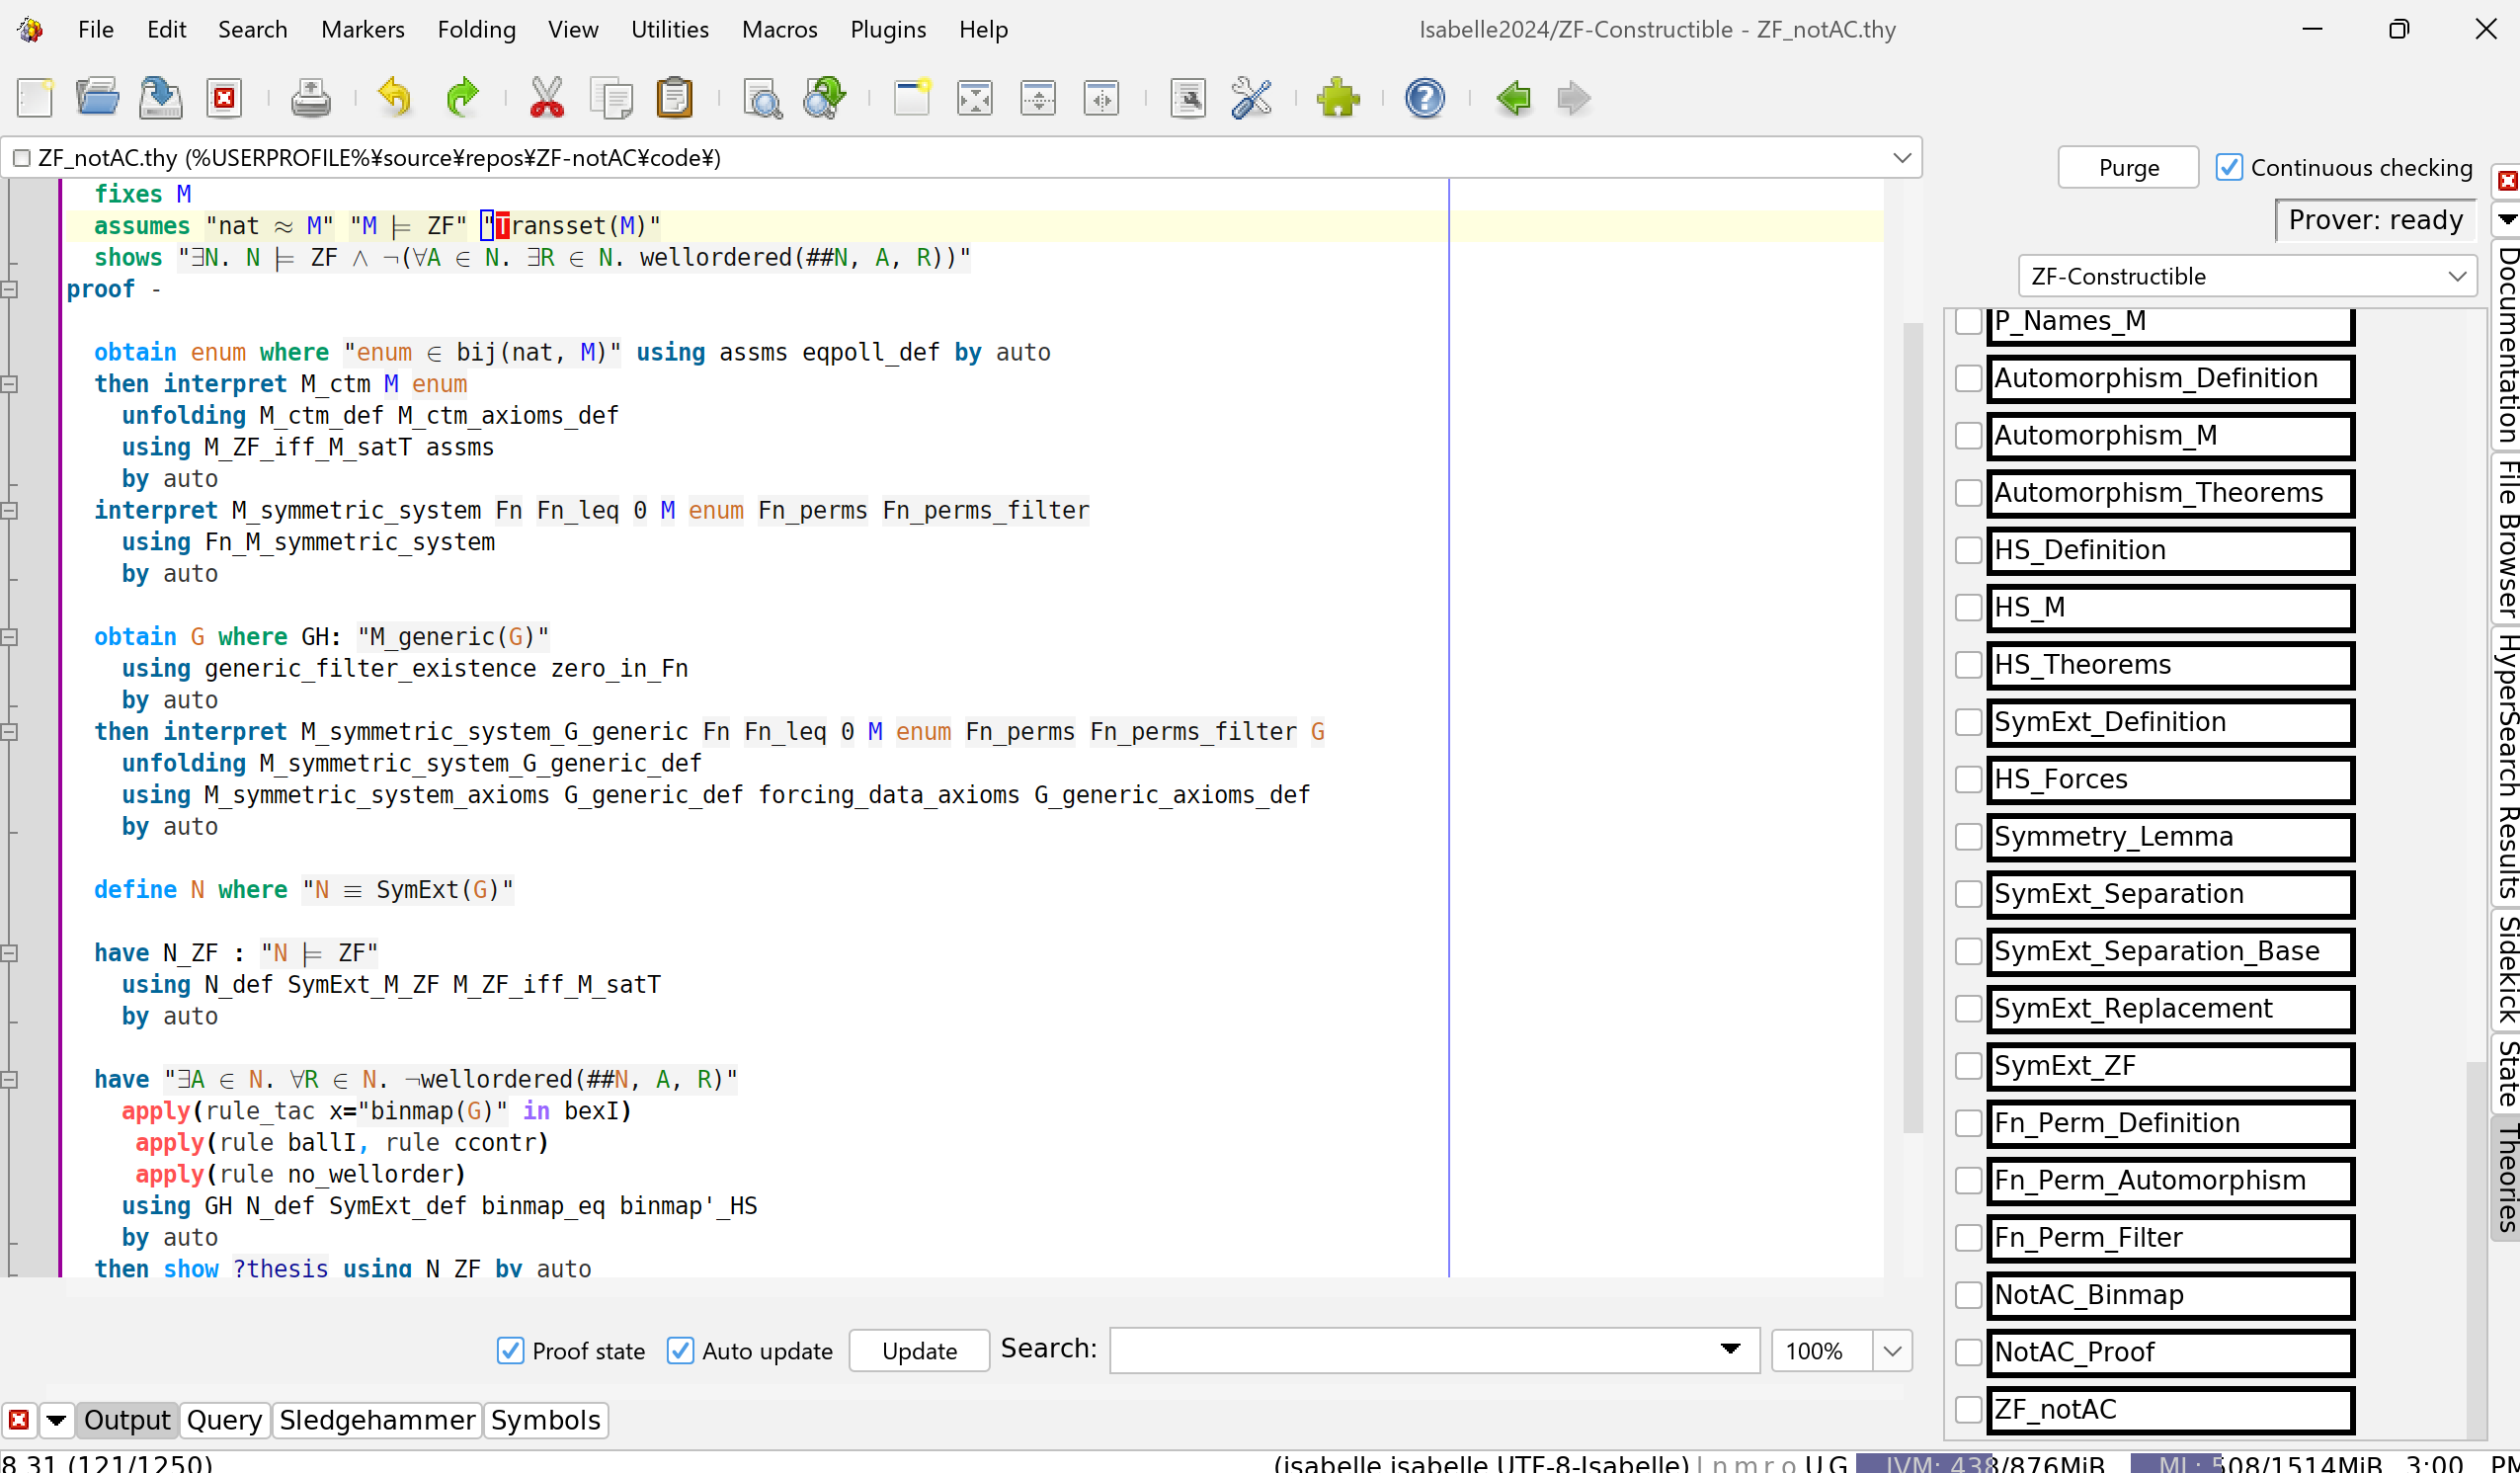
\includegraphics[width=1.0\linewidth]{./images/isabelle_editor.png}
            \end{figure}
            \vspace{-10pt}
            \begin{columns}
                \begin{column}{0.4\textwidth}
                    
\includegraphics[width=1\linewidth]{./images/lean.png}
                \end{column}
            \end{columns}
            \vspace{-10pt}
            \begin{columns}
                \begin{column}{0.4\textwidth}
                    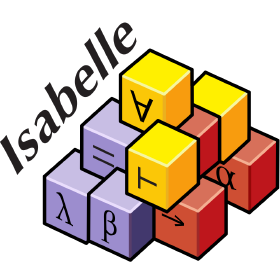
\includegraphics[width=1\linewidth]{./images/isabelle_logo.png}
                \end{column}
                \begin{column}{0.4\textwidth}
                    
\includegraphics[width=1\linewidth]{./images/coq.png}
                \end{column}
            \end{columns}
        \end{column}
    \end{columns}

    %----------------------------------------------
    % coqの画像 https://ja.wikipedia.org/wiki/Coq#/media/%E3%83%95%E3%82%A1%E3%82%A4%E3%83%AB:CoqProofOfDecidablityOfEqualityOnNaturalNumbers.png
    %----------------------------------------------

\end{frame}

%----------------------------------------------
%    マイクロカーネル
%    https://read.seas.harvard.edu/~kohler/class/cs260r-17/klein10sel4.pdf
%----------------------------------------------

\begin{frame}{Isabelle {\small [Paulson 86]}}
    \vspace{-5pt}
    \begin{itemize}[itemsep=3pt]
        \item 利用例 : \\
            seL4カーネルの形式検証 {\small \,[Klein et al. 14]}
            \vspace{-3pt}
            \begin{itemize}[itemsep=2pt]
                \item 130万行の証明
            \end{itemize}
        \item Archive of Formal Proofs
    \end{itemize}
    
    \begin{columns}
        \begin{column}{0.25\textwidth}
            \begin{figure}
                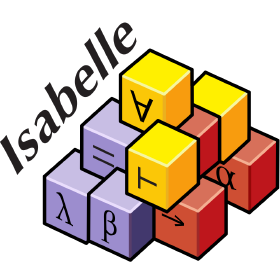
\includegraphics[width=0.7\linewidth]{./images/isabelle_logo.png}
            \end{figure}
        \end{column}
        \begin{column}{0.25\textwidth}
            \vspace{-7pt}
            \begin{figure}
                
\includegraphics[width=0.9\linewidth]{./images/sel4-logo.png}
            \end{figure}
        \end{column}
        \begin{column}{0.35\textwidth}
            \vspace{-20pt} 
            \begin{figure}
                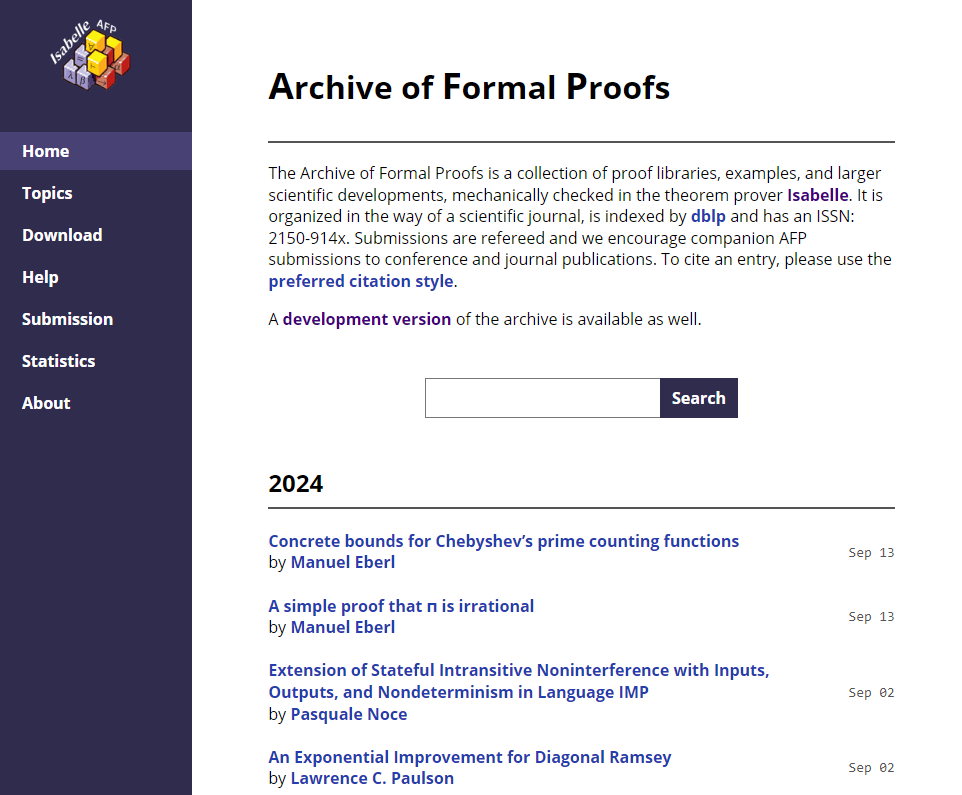
\includegraphics[width=0.8\linewidth]{./images/isabelle_archive.png}
            \end{figure}
        \end{column}
    \end{columns}
\end{frame}

\begin{frame}{Isabelle} \, \vspace{-30pt}
    {\small \begin{itemize}[itemsep=5pt]
        \item 論理体系「Pure」上で定理証明を行う
        \item Pure上に他の論理体系が構築されている
              \begin{itemize}
                  \item Higher-Order Logic
                  \item First-Order Logic 
              \end{itemize} 
              \vspace{-10pt}
        \item \textcolor{red}{Isabelle/ZF} : \\
        一階述語論理とZF(C)公理系のフレームワーク
    \end{itemize} 
    \vspace{-10pt}
    \hspace{-0.5cm}※本研究ではIsabelle/ZF上でさらに形式化されたZFを扱う(形式化されたZFのモデルとなっているような集合を構成する)
    }
\end{frame}

% 簡単な定理証明の例を紹介するといいかも
% apply-script, structured proofの説明

% ZFの公理を記述しているコードを紹介するといいかも
% https://isabelle.in.tum.de/dist/library/FOL/ZF/ZF_Base.html ZFの公理のコード

\begin{frame}{Isabelle/ZFにおける先行研究}
 
    {\small 
    \begin{itemize}[itemsep=8pt]
        \vspace{10pt}
        \item CHのZFC上の独立性証明{\small [Gunther et al. 20,22]}
            \vspace{3pt}
              {\small \begin{itemize}
                \item 強制法の形式化 (13K行)
                \item CHの独立性証明 (16K行) ※Leanにもある
              \end{itemize} }

        \item ACのZF上の相対的無矛盾性証明{\small [Paulson 02]}
              {\small \begin{itemize}
                      \item 構成可能宇宙を形式化 (12K行)
                  \end{itemize} }
              % https://arxiv.org/pdf/2001.09715 強制法の形式化
              % https://cs.famaf.unc.edu.ar/~pedro/forcing/Independence_CH/document.pdf CHの独立性証明
    \end{itemize}
    \begin{itemize}
        \item [\textcolor{red}{$\blacktriangleright$}] $\neg$ACの相対的無矛盾性証明は\\
        形式化されていなかったので挑戦
    \end{itemize}
    }
\end{frame}

\begin{frame}{本研究におけるIsabelle/ZFの利点}
    \begin{itemize}
        \item 集合論に関する補題・糖衣構文が豊富
        \item 強制法の形式化{\small [Gunther et al. 20]}が\\すでにある
        {\small \begin{itemize}[itemsep=15pt]
            \vspace{10pt}
            \item ZFのc.t.m.の存在を仮定している
            \begin{itemize}
                \item c.t.m. : countable transitive model
            \end{itemize}
            \item Lean3にも強制法の形式化があるが\\
            Lean3は開発終了
        \end{itemize}}
    \end{itemize}
    {\small ※一階述語論理の形式化は[Paulson 02]を利用}
\end{frame}


\section{証明概略}
\begin{frame}{証明概略 {\small [Karagila 23]}}
    \vspace{-4pt}
    ZFのc.t.m. $M$から出発して\\
    ZF+$\neg$ACのモデル$N$を構成する
    \vspace{-6pt}
    {\small 
    \begin{itemize}[itemsep=10pt]
        \item $N$はFirst Cohen Modelと呼ばれるモデル
        \begin{itemize}
            \item generic extensionの部分モデルである\\
            \textcolor{red}{symmetric extension}のひとつ
        \end{itemize}              
        \item $N$はZFを満たすが、整列可能定理を満たさない
        \vspace{3pt}
        \begin{itemize}
            \item $N \vDash $ 「単射$\omega \rightarrow A$がない無限集合$A$が存在」
            \begin{itemize}
                \item $N$ではこの$A$が整列できない
            \end{itemize}
        \end{itemize}
    \end{itemize}}
\end{frame}

\begin{comment}
    
\end{comment}

\section {Isabelle/ZFによる形式化}

\begin{frame}{成果}
    本研究で形式証明した命題
    \begin{figure}
        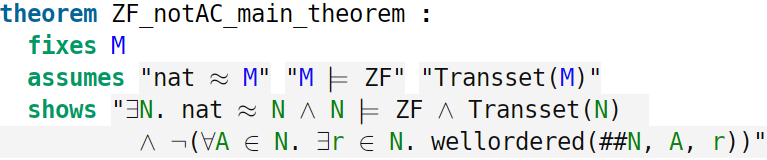
\includegraphics[width=\linewidth]{./images/ZF_notAC_main_theorem.png} 
    \end{figure} 
    \vspace{-15pt}
    意味 \\
    {\small
    \hspace{1cm}$M$をZFのc.t.m.とする。このとき \\
    \vspace{4pt}\hspace{1cm}あるZFのc.t.m. $N$があって \\
    \hspace{1cm}$N$は整列可能定理を満たさない
    }
\end{frame}

\begin{frame}{作業工程}
    以下の工程に分けられる
    {\small
    \begin{itemize}[itemsep=8pt,left=0.5cm]
        \item [1.] symmetric extensionの構成法の定義
        \item [2.] ZFのモデルであることの証明
        \item [3.] First Cohen Modelの構成
        \item [4.] それが$\neg$ACを満たすことの証明
    \end{itemize}
    }
\end{frame}

\begin{frame}{作業量}
    約1万5千行のコード \hspace{0.6cm} {\small 補題など(3K行)}
    {\small
    \begin{itemize}[itemsep=8pt,left=0.5cm]
        \item [1.] symmetric extensionの定義(3K行)
        \item [2.] ZFのモデルであることの証明(5K行)
        \item [3.] First Cohen Modelの構成(2K行)
        \item [4.] それが$\neg$ACを満たすことの証明(2K行)
    \end{itemize} 

    ※Isabelle/ZFでの集合論の形式化の各先行研究と同じくらい
    }
\end{frame}

\begin{frame}{面倒だった点\, {\normalsize 自明なことの確認が大変}}
    
    {\small\begin{itemize}[left=0cm,itemsep=8pt]
        \item クラスが本当にクラスであること
        \begin{itemize}
            \item 実際に論理式を構成する必要がある
        \end{itemize}
        \item 定義した関数が本当に関数であること
        \vspace{5pt}
        \begin{itemize}
            \item 特に「帰納的に定義された$M$内の関数」
            \vspace{5pt}
            {\begin{itemize}[itemsep=5pt]
                \item 仮定とZFからちゃんと\\
                構成できるか?
                \item このような関数を定義するための\\
                補題が2千行以上
            \end{itemize}}
        \end{itemize}
    \end{itemize}}
\end{frame}

\begin{comment}

\begin{frame}{困難だった点(2)\, {\normalsize 先行研究の強制関係の定義}}
    \begin{itemize}[itemsep=9pt]
        \item よくあるfor allに対する強制関係の定義
              $$ p \Vdash \forall x \phi(x, \dot{x_1}, ..., \dot{x_n}) \Leftrightarrow \forall \dot{x} \in M^\Pbb(p \Vdash \phi(\dot{x}, \dot{x_1}, ..., \dot{x_n})) $$
        \item 先行研究{\small [Gunther et al. 20]}の定義
              $$ p \Vdash \forall x \phi(x, \dot{x_1}, ..., \dot{x_n}) \Leftrightarrow \forall x \in \textcolor{red}{M}(p \Vdash \phi(x, \dot{x_1}, ..., \dot{x_n})) $$
              {\small 
                \hspace{0.5cm}※この定義でうまくいくように修正されている
              }
        \item [\textcolor{red}{$\blacktriangleright$}] 強制関係の帰納法に$M \setminus \Pbb$-name以外が混入する...
    \end{itemize}
\end{frame}
\begin{frame}{解決策(2)}
    \begin{itembox}[l]{先行研究{\small [Gunther et al. 20]}の$x_G$の定義}
    {\small
        $x \in M$に対し
        \vspace{-5pt}
        $$x_G := \{ y_G \, | \, y \in \bm{\mathbf{dom}}(x), \exists p \in G. (y, p) \in x \}$$
    }
    \end{itembox}
    \vspace{-1cm}
    {\small 
    \begin{itemize}[itemsep=4pt]    
        \item $x_G$が$M$上の関数になっている
        \item $x \in M$に対し、ある$\dot{z} \in M^\Pbb$があって$x_G = \dot{z}_G$
            \vspace{3pt}
              {\small
              \begin{itemize}
                  \item この事実を形式化し帰納法中で$x$の代わりに$\dot{z}$を使う
                  \item 最終的には解決策(3)で問題の帰納法自体不要に
              \end{itemize}}
    \end{itemize}
    }
\end{frame}

\end{comment}


\begin{frame}{困難だった点\, {\normalsize $N$がZFをみたすことの証明}}
    \vspace{-1pt}
    {\small 
    Isabelle/ZFで構成した$N$が$M[G]$において\\
    クラスであることが証明できなかった
    \begin{itemize}[left=0.1cm,itemsep=8pt]
        \item 書き下すのが面倒なだけでなく、非自明?
        \item これは[Karagila 23]で用いられている\\
        次の命題の証明に必要
    \end{itemize}
    \vspace{-0.2cm}
    \begin{itembox}[l]{命題}
        {\small
            $N$が推移的かつalmost universalなクラスで\\
            $\Delta_0$-separationを満たすならば
            $N$はZFの内部モデルである
        }
    \end{itembox} 
    }
\end{frame}

\begin{frame}{解決策}
    \vspace{-50pt}
    {\small
        \begin{itemize}[itemsep=8pt]
            \item $\bm{\mathbf{HS}}$に相対化した強制関係$\textcolor{red}{\Vdash_{\bm{\mathbf{HS}}}}$を形式化
                  \begin{itemize}[left=0cm]
                      \item 参考資料[Karagila 23]に書かれている概念
                      \item 強制関係の定義の量化の動く範囲を$\bm{\mathbf{HS}}$に制限
                      \item $\Vdash_{\bm{\mathbf{HS}}}$は、symmetric extensionに対し、\\
                            generic extensionに対する$\Vdash$のように振舞う
                  \end{itemize}
            \item $\Vdash_{\bm{\mathbf{HS}}}$を用いてZFのモデルであることを証明
                 % \begin{itemize}
                 %     \item 強制関係の帰納法が不要になり{\footnotesize「困難だった点(2)」}も解決
                 % \end{itemize}
        \end{itemize}
    }
    \begin{textblock*}{0.58\linewidth}(0pt, 190pt)
        \begin{figure}
            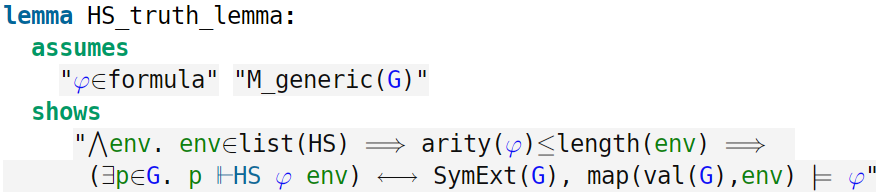
\includegraphics[width=\linewidth]{./images/HS_truth_lemma.png}
        \end{figure}
    \end{textblock*}
    \begin{textblock*}{0.58\linewidth}(183pt, 190pt)
        \begin{figure}
            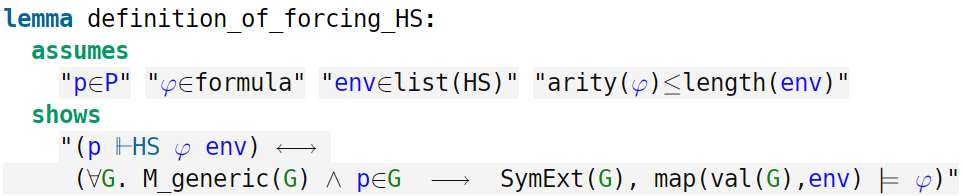
\includegraphics[width=\linewidth]{./images/HS_forces_def.png}
        \end{figure}
    \end{textblock*}
\end{frame}


\section {考察}

\begin{frame}{考察(1) {\normalsize c.t.m.アプローチについて}}
    \vspace{-30pt}
    \,{\small 
    \begin{itemize}
        \item 本研究で形式化したのは、\\
              「ZFのc.t.m.が存在 $\rightarrow$ ZF+$\neg$ACのc.t.m.が存在」
              \vspace{5pt}
              \begin{itemize}
                \item ZFのc.t.m.の存在は、強制法の形式化[Gunther et al. 20]を使うため仮定
              \end{itemize}
        \item 証明したいのはCon(ZF)$\rightarrow$Con(ZF+$\neg$AC)だが、\\
              ZFのc.t.m.の存在は、Con(ZF)から証明できない
              \vspace{5pt}
              \begin{itemize} 
                \item このギャップを埋める部分が形式化できていない(本当は形式化したい)
              \end{itemize}
    \end{itemize}
    }
\end{frame}

\begin{frame}{形式化できていない部分}
    \vspace{-2pt}
    {\small 
        以下の形式化ができれば、\\ZFのc.t.m.の存在の仮定をなくせる
        \vspace{-4pt}
        \begin{itemize}
            \item 任意のZFの有限部分$\Delta$に対し、ZFの有限部分$\Gamma$\\
                  があって$\Gamma$のc.t.m.が存在すれば$\Delta + \neg$ACの\\
                  モデルが存在する
                  \begin{itemize}
                    \item 今回の形式化を修正すれば可能
                  \end{itemize}
        \vspace{-14pt}
        \item ZFの有限部分$\Gamma$に対し、$\Gamma$のc.t.m.が存在する
                  \begin{itemize}[itemsep=5pt]
                    \item ZFモデルの中でZFのモデルを考える必要がある?
                    \item 形式化が難しい?
                  \end{itemize}
                \end{itemize}
    }
\end{frame}

\begin{frame}{考察(2) メタ/対象レベル}
    \hspace{-0.5cm}ZFのモデルの中の性質の証明が大変だった
    \hspace{-0.5cm}{\small 
    \begin{itemize}[itemsep=5pt, left=0cm]
        \item コード化された論理式を扱う必要があった
        \item メタレベルで成り立つことを\\
              もう一度証明しなければいけなかった
        \item [\textcolor{red}{\blacktriangleright}]
        メタ/対象レベルの証明を同時に書ける or \\
        他方に変換できるような機能があると便利
        \item [\textcolor{red}{\blacktriangleright}]
        今回のテーマに限らず\\数学基礎論の形式化でも有用
    \end{itemize}}
\end{frame}

\begin{frame}{まとめ}
    \begin{center}
        $\neg$ACの相対無矛盾性証明を\\
        Isabelle/ZFで形式化
    \end{center}
    {\small
    \begin{itemize}[itemsep=8pt]
        \item ZFのc.t.m.から出発し、\\ZF+$\neg$ACをみたすsymmetric extensionを構成
        \item c.t.m.に関する形式化できていない部分がある
        \item 参考資料の通りにいかず試行錯誤した部分も
        \item メタ/対象レベルの形式的証明を「つなげる」\\機能がほしい
    \end{itemize}
    }
\end{frame}

\appendix
\setbeamertemplate{footline}{}
 
\begin{frame}{参考文献(1)}
    \vspace{-30pt}
    \, {\footnotesize 
    \begin{itemize}[itemsep=5pt, left=0pt]
        \item K. Kunen, Set Theory An Introduction To Independence Proofs, North-Holland, 1980 \\
              日本語訳: 藤田 博司 訳, 集合論: 独立性証明への案内, 日本評論社, 2008
        \item T. Jech, Set Theory: The Third Millennium Edition, Springer, 2002
        \item T. Jech, The Axiom of Choice, Dover Publications, 2008
        \item A. Karagila, Lecture Notes: Forcing \& Symmetric Extensions, 2023
    \end{itemize}
    }

\end{frame}

\begin{frame}{参考文献(2)}
    \vspace{-30pt}
    \, {\footnotesize 
    \begin{itemize}[itemsep=5pt, left=0pt]
        \item G. Klein et al., seL4: Formal Verification of an OS Kernel, 2014
        \item LC. Paulson, The Relative Consistency of the Axiom of Choice Mechanized Using Isabelle/ZF, 2003
        \item E. Gunther et al., Formalization of Forcing in Isabelle/ZF, 2020
        \item E. Gunther et al., The Independence of the Continuum Hypothesis in Isabelle/ZF, 2022
    \end{itemize}
    }

\end{frame}

\begin{comment}
    \item K. Kunen, Set Theory An Introduction To Independence Proofs, North-Holland, 1980\\
              日本語訳: 藤田 博司 訳, 集合論: 独立性証明への案内, 日本評論社, 2008
        \item T. Jech, Set Theory: The Third Millennium Edition, Springer, 2002
        \item T. Jech, The Axiom of Choice, Dover Publications, 2008
        \item A. Karagila, Lecture Notes: Forcing & Symmetric Extensions, 2023
        \item G. Klein et al., seL4: Formal Verification of an OS Kernel, 2014
        \item LC. Paulson, The Relative Consistency of the Axiom of Choice Mechanized Using Isabelle/ZF, 2003
        \item E. Gunther et al., Formalization of Forcing in Isabelle/ZF, 2020
        \item E. Gunther et al., The Independence of the Continuum Hypothesis in Isabelle/ZF, 2022
\end{comment}

\end{document}


